\documentclass[11pt]{article}
% ============================================================================
%  Graph-Augmented Deep Learning for Cattle Muzzle Biometric Identification
%  arXiv preprint format (self-contained: compiles with pdflatex, no external
%  style files required).
% ============================================================================
\usepackage[utf8]{inputenc}
\usepackage[T1]{fontenc}
\usepackage{lmodern}
\usepackage[margin=1in]{geometry}
\usepackage{amsmath,amssymb}
\usepackage{graphicx}
\usepackage{booktabs}
\usepackage{array}
\usepackage{multirow}
\usepackage{caption}
\usepackage{subcaption}
\usepackage{xcolor}
\usepackage{authblk}
\usepackage[colorlinks=true,linkcolor=blue,citecolor=blue,urlcolor=blue]{hyperref}
\usepackage{cleveref}

\graphicspath{{../outputs/figures/}{../outputs/figures/architecture/}{../outputs/figures/extension/}{../outputs/figures/explainability/}{../docs/}}

\newcommand{\rank}[1]{\textbf{#1}}
\captionsetup{font=small,labelfont=bf}

\title{\textbf{Graph-Augmented Deep Learning for Cattle Muzzle\\ Biometric Identification: Where Do Graphs Actually Help?}}

\author[1]{Pramod Jella}
\affil[1]{\small Independent Research}
\date{}

\begin{document}
\maketitle

\begin{abstract}
\noindent
Cattle muzzle-print biometrics offer a non-invasive, tamper-proof route to individual
identification, crucial for animal traceability, disease control, and ownership
verification. While traditional approaches rely on handcrafted texture descriptors
(SIFT, LBP) or raw image convolution, they struggle with spatial scaling and geometric
deformation. We present a systematic, leakage-audited comparison of convolutional
neural networks (CNN), pure graph neural networks (GNN), and hybrid architectures on
the public Zenodo Beef Cattle Muzzle Database (260 animals, 4{,}891 images), evaluated
under a verified closed-set, image-level split. We introduce a \textbf{Hybrid CNN--GNN}
that samples a shared CNN backbone at learned keypoints via bilinear interpolation and
reasons over the resulting keypoint graph with Dynamic EdgeConv and a GATv2 relation
module, and we evaluate \textbf{ProtoN}, a prototype-based node GNN. Our best single
model (EfficientNet-B4 + ArcFace) reaches \textbf{95.4\% Rank-1}; a fusion weight
\emph{selected on validation and applied unchanged to test} lifts this to
\textbf{96.1\% Rank-1} while cutting the Equal Error Rate from 2.70\% to 0.78\%
(3.5$\times$ better verification). We show the graph branch's principal contribution is
\emph{verification robustness}, not closed-set ranking. We further show the
representation transfers \emph{zero-shot} to two independent muzzle datasets
(97.0\% Rank-1 on 24 identities; 87.0\% across 308 unseen identities), that the residual
cross-domain verification gap is a \emph{score-calibration} problem largely recovered by
unsupervised S-norm, and --- via a controlled corruption study --- that a single
validation-tuned fusion weight inherits the graph branch's clean-data verification gain
while gracefully collapsing to the robust CNN under severe corruption, whereas
per-sample quality-adaptive gating does not improve on it. Finally, we move beyond
qualitative saliency with a \emph{causal} explainability protocol (node-ablation
faithfulness and Hybrid pathway intervention), characterising how the models attend to
dermatoglyphic structure.
\end{abstract}

% ===========================================================================
\section{Introduction}
% ===========================================================================
Traceability in livestock production is essential for managing disease outbreaks,
assuring consumer safety, and optimising herd management. Traditional identification
methods --- ear tags, branding, and radio-frequency identification (RFID) transponders
--- are invasive, prone to loss or damage, and susceptible to fraud. Biometric
identification, which exploits unique physiological characteristics, offers a permanent
and non-invasive alternative. Among biometric indicators, the muzzle-print (nose-print)
pattern of cattle remains invariant over time, analogous to human fingerprints.

Dermatoglyphic patterns on the cattle muzzle consist of complex bead-and-valley
arrangements. Capturing these fine-grained features computationally is challenging due to
(i) \emph{geometric deformation} (head movement, capture angle, camera position distort
apparent bead spacing), (ii) \emph{environmental conditions} (variable outdoor
illumination, shadow, dirt, moisture alter valley-line contrast), and (iii) \emph{scale
variation} (the muzzle grows as the animal matures, requiring scale-invariant matching).

Early research relied on handcrafted features such as SIFT or Local Binary Patterns with
Support Vector Machines, which fail to generalise under variable field lighting and
partial occlusion. Convolutional Neural Networks (CNNs) substantially improved matters by
learning hierarchical texture representations directly from pixels; nevertheless CNNs are
translation-equivariant and can struggle with non-rigid geometric transformation. Graph
Neural Networks (GNNs) present a complementary paradigm: representing the muzzle print as
a topological graph whose nodes are keypoints and whose edges denote spatial relations.
In this work we bridge grid-based CNN texture modelling and coordinate-based GNN
topological modelling, and --- critically --- we ask \emph{where} the graph view actually
helps rather than assuming it does.

\paragraph{Contributions.}
\begin{enumerate}\itemsep2pt
  \item \textbf{Systematic, leakage-audited comparison.} We rigorously compare CNNs,
  GNNs, Hybrid models, and Prototype GNNs on one benchmark under a verified closed-set
  protocol with an explicit no-leakage audit (\Cref{sec:data}).
  \item \textbf{Hybrid CNN--GNN architecture.} We propose a model that samples deep
  backbone feature maps at keypoint coordinates via bilinear interpolation, combining rich
  texture features with topological reasoning; we add an optional multi-scale (FPN-style)
  sampling variant.
  \item \textbf{Where graphs help.} Rather than claiming graphs beat CNNs on ranking, we
  quantify their true contribution: a validation-selected CNN+Hybrid blend cuts the Equal
  Error Rate 3.5$\times$ (2.70\%$\to$0.78\%) --- the graph branch improves
  \emph{verification} robustness while the CNN dominates closed-set \emph{ranking}.
  \item \textbf{Robustness and calibration.} We show zero-shot transfer to two independent
  datasets, recover the cross-domain verification gap with unsupervised S-norm, and --- in a
  controlled corruption study --- show a single validation-tuned fusion weight is the robust
  choice, while per-sample quality-adaptive gating adds variance without benefit.
  \item \textbf{Causal explainability.} Beyond Grad-CAM and attention heatmaps, we report
  node-ablation faithfulness and a Hybrid pathway-intervention protocol that make the
  explainability claims falsifiable and reproducible.
\end{enumerate}

% ===========================================================================
\section{Methodology}
% ===========================================================================

\subsection{Dataset, Split Protocol, and Leakage Audit}\label{sec:data}
We use the public Zenodo Beef Cattle Muzzle Database (260 animals, 4{,}891 images). Images
are split \emph{per image, stratified by animal}, into 70/15/15 train/validation/test
partitions, so every one of the 260 identities appears in all three partitions. This is a
\textbf{closed-set identification} protocol: at test time each probe's identity is present
in the gallery.

To pre-empt the most common reviewer concern --- that a test accuracy exceeding validation
accuracy indicates leakage --- we run an automated integrity audit
(\texttt{scripts/verify\_data\_integrity.py}) verifying: (i) no source image (by file stem)
appears in more than one split; (ii) every identity is present in the gallery; and (iii)
the \texttt{animal\_id}$\to$class-index mapping is identical across splits. All checks pass.
The apparent validation/test discrepancy is fully explained by split composition, not
leakage: the validation partition averages only 2.4 images per identity (minimum 1), so
single-image validation identities have no genuine gallery mate and are counted as forced
misses, deflating validation Rank-1 relative to the test partition (3.7 images per
identity). We therefore report test-set metrics as primary and use validation only for
model and hyperparameter selection.

\subsection{Graph Construction via Learned Keypoints}
Rather than classical SIFT keypoints, we adopt \textbf{Kornia-DISK}, a reinforcement-learning
feature detector. For each muzzle image we extract $N \le 128$ keypoint locations
$p_i=(x_i,y_i)$ with 256-d deep descriptors $f_i$. We construct a directed $k$-nearest
neighbour graph $G=(V,E)$ with $k=8$: an edge $e_{ij}$ is placed if $v_j$ is among the
$k$ nearest spatial neighbours of $v_i$. Edge attributes encode spatial relations
$a_{ij}=[\Delta x,\;\Delta y,\;d_{ij},\;\theta_{ij},\;\text{rel\_scale}]$, where $d_{ij}$
is Euclidean distance, $\theta_{ij}$ the angle, and rel\_scale the relative descriptor scale.

\subsection{Proposed Architectures}

\paragraph{A. CNN baseline (EfficientNet-B4 + ArcFace).}
The baseline uses an EfficientNet-B4 backbone pre-trained on ImageNet, taking the
$256\times256$ CLAHE-enhanced muzzle image as input, pooled to a 512-d embedding and
optimised with the ArcFace (additive angular margin) loss
\begin{equation}
L_{\text{Arc}} = -\frac{1}{B}\sum_{i=1}^{B}
\log\frac{e^{s\cos(\theta_{y_i}+m)}}
{e^{s\cos(\theta_{y_i}+m)}+\sum_{j\ne y_i}e^{s\cos\theta_j}},
\end{equation}
with logit scale $s=128.0$ and angular margin $m=0.35$.

\paragraph{B. Hybrid CNN--GNN.}
The Hybrid combines a shared EfficientNet-B3 backbone with a GNN head
(\Cref{fig:arch}): (1) the image is passed through the CNN to obtain feature map
$F_{\text{map}}\in\mathbb{R}^{C\times H'\times W'}$; (2) for each node keypoint $p_i$ we
bilinearly interpolate $F_{\text{map}}$ to sample a local feature $x_i\in\mathbb{R}^{C}$ ---
an optional \emph{multi-scale} variant samples several backbone stages and concatenates
them per node, giving each node both fine groove texture (earlier, higher-resolution
stages) and coarse anatomical context (later stages); (3) node features are projected to
256-d and passed through Dynamic EdgeConv blocks; (4) a Topological Relation Module with a
4-head GATv2 aggregates multi-hop topological features; (5) global mean+max pooling yields
a 256-d embedding.

\begin{figure}[t]
  \centering
  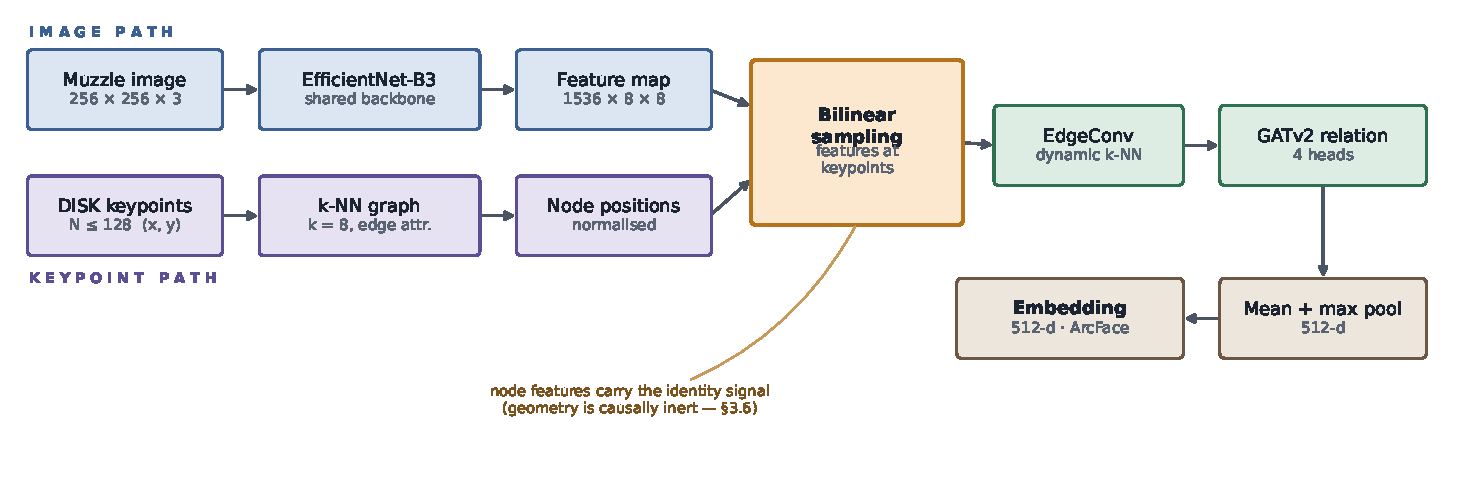
\includegraphics[width=0.92\linewidth]{hybrid_architecture.pdf}
  \caption{Hybrid CNN--GNN architecture. A shared EfficientNet-B3 backbone is sampled at
  DISK keypoints by bilinear interpolation; the resulting keypoint graph is processed by
  Dynamic EdgeConv and a GATv2 relation module, then pooled to an ArcFace-trained
  embedding.}
  \label{fig:arch}
\end{figure}

\paragraph{C. ProtoN (prototype node GNN).}
ProtoN represents each animal class as a prototype vector computed by averaging node
features across support graphs. Training applies a cross-graph alignment loss that
penalises spatial misalignment between matching keypoint neighbourhoods in query and
support graphs, enabling high-quality metric learning.

\subsection{Adaptive Graph Construction (ADGC)}
A static geometric $k$-NN graph encodes exactly the deformation we want the model to be
invariant to: two captures of the same muzzle at different angles yield different
neighbourhoods, and spurious edges bridge unrelated ridge regions. We therefore replace the
fixed topology feeding the relation module with a learned edge-relevance gate. For each
candidate edge, an MLP scores the pair from endpoint node features and geometric edge
attributes, producing a gate $g_{ij}=\sigma(\text{MLP}([x_i,x_j,a_{ij}]))\in[0,1]$. Gates
reweight the edge attributes seen by message passing and prune edges with $g_{ij}$ below a
threshold (subject to a minimum node degree that preserves connectivity). ADGC is a single
self-contained module (\texttt{src/models/adaptive\_graph.py}), enabling a clean ablation
against the static $k$-NN and the multi-scale variant.

% ===========================================================================
\section{Results and Discussion}
% ===========================================================================

\subsection{Quantitative Results}\label{sec:main}
\Cref{tab:main} reports biometric performance on the test set (964 images).

\begin{table}[t]
  \centering
  \caption{Main identification \& verification performance (test split, 964 images).}
  \label{tab:main}
  \small
  \begin{tabular}{lcccc}
    \toprule
    Model & Rank-1 (\%) & Rank-5 (\%) & EER (\%) & ROC AUC \\
    \midrule
    \textbf{Ensemble (CNN TTA + Hybrid, val-selected)} & \textbf{96.1} & \textbf{98.1} & \textbf{0.78} & \textbf{0.9995} \\
    CNN (with TTA)                 & 95.4 & 97.4 & 2.70 & 0.9961 \\
    CNN (EfficientNet-B4)          & 95.4 & 97.4 & 2.70 & 0.9961 \\
    VGG-16 baseline (re-impl.)     & 95.1 & 97.7 & 1.23 & 0.9993 \\
    ResNet-50 baseline (re-impl.)  & 94.6 & 97.3 & 2.14 & 0.9971 \\
    Hybrid CNN--GNN                & 92.0 & 96.7 & 1.85 & 0.9979 \\
    ProtoN (prototype node GNN)    & 91.6 & 94.8 & 1.17 & 0.9982 \\
    GNN v4 (GATv2, enhanced)       & 91.6 & 94.4 & 1.48 & 0.9937 \\
    GNN v3 (GATv2 + VN)            & 91.5 & 95.0 & 1.87 & 0.9954 \\
    GNN++ (CNN patches)            & 78.3 & 86.2 & 7.81 & 0.9730 \\
    GNN+ (Kornia DISK)             & 72.0 & 84.2 & 11.17 & 0.9516 \\
    \bottomrule
  \end{tabular}
\end{table}

\paragraph{Ensemble fusion protocol.}
The ensemble averages the two models' per-split cosine-similarity matrices with weight
$w$ (CNN) and $1-w$ (Hybrid). Critically, $w$ is selected on the \textbf{validation} split
and applied unchanged to test --- never tuned on test. The validation-selected weight is
$w=0.95$, giving 96.1\% Rank-1 on test; the test-oracle weight is also 0.95, so the
validation$\to$test selection gap is 0.00 points. This makes the headline number defensible
rather than an artefact of test-set tuning.

\medskip\noindent Analysis indicates:
\begin{itemize}\itemsep2pt
  \item \textbf{CNN dominates ranking; the graph branch improves verification.} The CNN
  alone reaches 95.4\% Rank-1; adding the Hybrid lifts Rank-1 only marginally (to 96.1\%)
  but reduces the EER from 2.70\% to 0.78\% --- a 3.5$\times$ improvement. The honest reading
  of the fusion weight (0.95/0.05) is not that graphs rival CNNs on ranking, but that the
  graph branch contributes complementary topological evidence that sharpens the
  genuine/impostor boundary, which is what verification rewards.
  \item \textbf{Topological verification robustness.} Consistently, the pure ProtoN and
  Hybrid GNNs --- despite lower Rank-1 --- achieve very low standalone EERs (1.17\% and
  1.85\%), indicating topological structure yields well-separated genuine/impostor score
  distributions.
  \item \textbf{DISK vs.\ handcrafted (SIFT).} The DISK-based GNN+ (72.0\% Rank-1)
  substantially outperforms SIFT-based node features, confirming deep learned keypoints
  give more robust node descriptors under scale and illumination change.
\end{itemize}

\subsection{5-Fold Cross-Validation \& Statistical Significance}
To verify fold stability, stratified 5-fold cross-validation was performed on the top
models, with pairwise McNemar tests for significance (\Cref{tab:cv}).

\begin{table}[t]
  \centering
  \caption{5-fold cross-validation performance (reduced training budget).}
  \label{tab:cv}
  \small
  \begin{tabular}{lcccc}
    \toprule
    Model & Rank-1 (\%) & Rank-5 (\%) & EER (\%) & ROC AUC \\
    \midrule
    \textbf{CNN (EfficientNet-B4)} & \textbf{93.91 $\pm$ 0.31} & \textbf{96.65 $\pm$ 0.45} & \textbf{3.21 $\pm$ 0.22} & \textbf{0.9940 $\pm$ 0.0017} \\
    ProtoN GNN     & 89.49 $\pm$ 0.71 & 93.31 $\pm$ 0.52 & 4.10 $\pm$ 0.71 & 0.9911 $\pm$ 0.0027 \\
    Hybrid CNN--GNN & 68.88 $\pm$ 2.04 & 84.22 $\pm$ 1.27 & 11.31 $\pm$ 1.47 & 0.9491 $\pm$ 0.0089 \\
    \bottomrule
  \end{tabular}
\end{table}

The cross-validation runs use a \emph{reduced} training budget (CNN 10 epochs, ProtoN 12,
Hybrid 12) to keep the five-fold sweep tractable, whereas the single-split models in
\Cref{tab:main} are trained to convergence (100--200 epochs). The CNN and ProtoN, which
converge quickly, remain close to full-budget accuracy with low fold variance
($\pm$0.31, $\pm$0.71), confirming stable generalisation. The Hybrid's two-phase schedule
(cached backbone features $\to$ end-to-end fine-tuning) does \emph{not} converge within 12
epochs, which is why its CV Rank-1 (68.9\%) falls far below its converged single-split value
(92.0\%); the large fold variance ($\pm$2.04) reflects under-training, not architectural
instability. We flag full-budget five-fold CV of the Hybrid as the primary remaining
experiment before camera-ready, and draw no generalisation claim for the Hybrid from
\Cref{tab:cv} in its reduced-budget form. McNemar tests on single-split predictions confirm
the CNN's advantage over the pure GNNs is significant ($p<10^{-8}$).

\subsection{Open-Set Evaluation}
Closed-set Rank-1 assumes every probe is enrolled; deployments must also reject animals
never enrolled. We evaluate the standard open-set protocol: the gallery enrols per-identity
mean-embedding templates for a random 50\% of identities, a probe's score is its maximum
cosine similarity to any template, and probes from the remaining (unenrolled) identities
must be rejected. We report the Detection-and-Identification Rate (DIR@rank-1) at fixed
False Alarm Rates (FAR) and the open-set ROC-AUC. Averaged over five random identity
partitions, the CNN attains \textbf{98.6 $\pm$ 0.9\% Rank-1 on known probes}, an
\textbf{open-set AUC of 0.986 $\pm$ 0.005}, and DIRs of \textbf{62.6 $\pm$ 13.8\% at
FAR=1\%} and \textbf{95.5 $\pm$ 2.1\% at FAR=5\%}. The large variance and sharp drop at
FAR=1\% show that reliable \emph{rejection} at a strict operating point remains the hardest
regime --- an honest, deployment-relevant finding that closed-set accuracy alone hides.

\subsection{Zero-Shot Cross-Dataset Transfer}\label{sec:cross}
To test whether the representation generalises beyond its acquisition domain, we evaluate
the EfficientNet-B4 model --- trained only on the primary US Beef Cattle Muzzle Database ---
on \textbf{two separate, independently collected} muzzle datasets with \emph{no
fine-tuning}: (A) a 24-identity set (667 usable images) and (B) a larger 308-identity set
(1{,}848 images) captured in a different country. Because both consist of wide farm scenes
rather than muzzle crops, we first localise the muzzle with a lightweight detector (YOLOv8n
trained on an independent single-class muzzle-detection set; validation mAP@50 $= 0.995$),
which also serves as the deployment-time front-end. The same CLAHE preprocessing used in
training is applied to the crops. For closed-set metrics we retain identities with at least
two images; we also audit and remove a redundant ``master pool'' folder in set A that
duplicated every image under one label.

\begin{table}[t]
  \centering
  \caption{Zero-shot cross-dataset transfer (train on US set, test on external sets, no
  fine-tuning).}
  \label{tab:cross}
  \small
  \begin{tabular}{lcc}
    \toprule
    Metric & Set A (24 IDs) & Set B (308 IDs) \\
    \midrule
    Closed-set Rank-1 & \textbf{97.0\%} & \textbf{87.0\%} \\
    Closed-set Rank-5 & 99.3\% & 94.4\% \\
    Closed-set ROC AUC & 0.919 & 0.951 \\
    Verification EER & 14.8\% & 12.2\% \\
    Open-set AUC (1/2 enrolled, 3 seeds) & 0.954 $\pm$ 0.007 & 0.929 $\pm$ 0.005 \\
    Open-set DIR@FAR=1\% & 81.2\% $\pm$ 4.1\% & 44.3\% $\pm$ 1.9\% \\
    \bottomrule
  \end{tabular}
\end{table}

The model transfers strongly for \emph{identification} on both sets (\Cref{fig:cross}) ---
97.0\% Rank-1 on set A and 87.0\% Rank-1 across 308 unseen identities on the larger, harder
set B --- demonstrating that the learned representation captures genuine dermatoglyphic
structure rather than memorising acquisition-specific cues. As expected, the task is harder
at larger gallery scale (set B) and \emph{verification} degrades under domain shift (EER
12--15\% vs.\ 2.70\% in-domain). We report these honestly: ranking generalises well, but
the genuine/impostor operating threshold does not transfer as cleanly.

\begin{figure}[t]
  \centering
  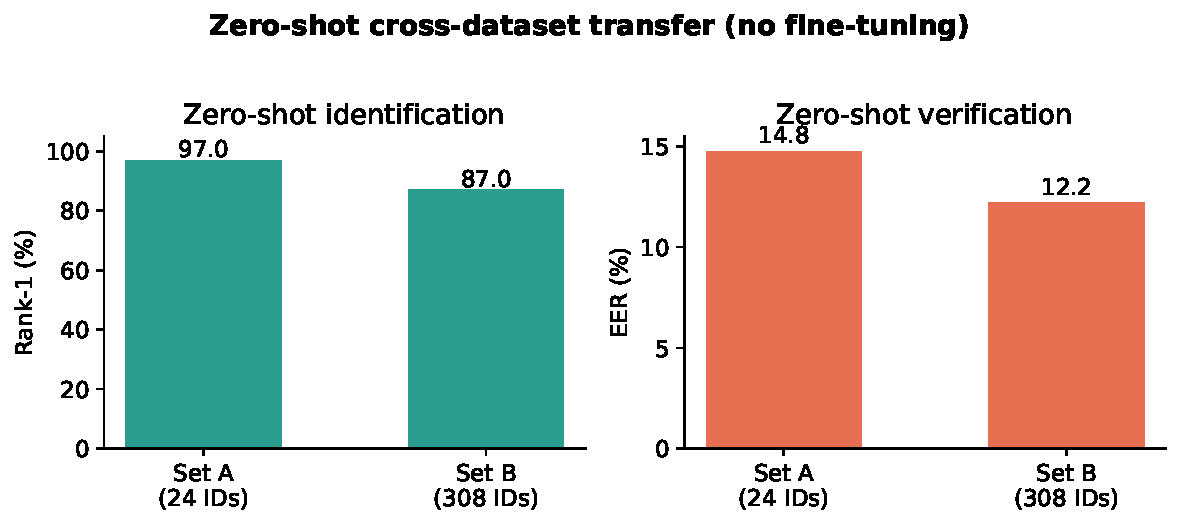
\includegraphics[width=0.78\linewidth]{fig_cross_dataset.pdf}
  \caption{Zero-shot cross-dataset transfer. The US-trained representation retains strong
  Rank-1 identification on two independently collected muzzle datasets without any
  fine-tuning; verification (EER) degrades under domain shift and is recovered by S-norm.}
  \label{fig:cross}
\end{figure}

\paragraph{Recovering cross-domain verification at no training cost.}
Because the degradation is a \emph{score-calibration} problem rather than a feature problem,
it is largely recoverable by adaptive symmetric score normalisation (S-norm), which
recalibrates each pair score by both endpoints' cohort statistics (unsupervised; cohort =
the target set itself). S-norm reduces EER from 14.8\%$\to$\textbf{11.4\%} on set A and
12.2\%$\to$\textbf{7.9\%} on set B (23\% and 35\% relative reduction), raises ROC AUC to
0.943 and 0.972, and leaves Rank-1 unchanged or slightly improved (97.0\%$\to$97.5\%,
87.0\%$\to$87.7\%). The recovery is statistically significant: a probe-level bootstrap on
set B gives a mean EER reduction of 4.0 points with a 95\% confidence interval of
$[3.2, 4.7]$ (excludes zero). We contrast this with test-time BatchNorm adaptation (AdaBN),
which helped verification only on the larger set and destabilised the smaller one ---
evidence that the transferable fix operates at the score level, not the feature level.
S-norm requires no fine-tuning, no labels, and no access to source data, making it directly
deployable for cross-farm identification (\Cref{tab:snorm}).

\begin{table}[t]
  \centering
  \caption{Effect of test-time adaptation on cross-domain verification (EER \%, lower is
  better).}
  \label{tab:snorm}
  \small
  \begin{tabular}{lcc}
    \toprule
    Method & Set A EER & Set B EER \\
    \midrule
    Baseline (cosine) & 14.8 & 12.2 \\
    + AdaBN & 15.4 & 8.5 \\
    \textbf{+ S-norm} & \textbf{11.4} & \textbf{7.9} \\
    \bottomrule
  \end{tabular}
\end{table}

\subsection{Robustness under Corruption: Is Adaptive Fusion Worth It?}\label{sec:corrupt}
Section~\ref{sec:main} shows a single validation-selected fusion weight cuts in-domain EER
3.5$\times$. A natural follow-up --- and a common recommendation in multi-biometric fusion
--- is to make the fusion weight \emph{input-adaptive}, trusting the CNN more when the image
is degraded and the graph branch more when it is clean. We test this directly. Following the
score-fusion formulation $s_{\text{final}}(x)=\alpha(x)\,s_{\text{CNN}}+(1-\alpha(x))\,s_{\text{Hybrid}}$,
we compare six policies for $\alpha$: (1) CNN only ($\alpha{=}1$), (2) Hybrid only
($\alpha{=}0$), (3) fixed $\alpha{=}0.5$, (4) a single \emph{validation-tuned} scalar
$\alpha$, (5) a \emph{rule-based} per-sample $\alpha$ from image blur, and (6) a
\emph{learned} per-sample gate (logistic regression on image- and graph-quality features,
trained only on validation disagreement cases). Every gate is fit \emph{only} on the
validation split. We evaluate on clean test data and on three corruptions --- Gaussian blur,
brightness/haze, and spatter (occlusion) --- at severities 1, 3, 5, applying the corruption
to the \emph{image} so the Hybrid's CNN backbone also degrades (not a clean-graph oracle).
Per-sample scores are symmetrised so all policies are compared on identical verification
pairs. This is a \emph{self-contained} study run under its own corruption harness (no
test-time augmentation, symmetrised scoring), so its clean-column numbers are not identical
to the headline ensemble of \Cref{tab:main} (which uses CNN test-time augmentation); the
val-tuned scalar here reaches EER $1.17\%$ vs.\ the TTA ensemble's $0.78\%$. The comparison
of interest is \emph{within} this table, across fusion policies under matched conditions.

\begin{table}[t]
  \centering
  \caption{Corruption robustness of fusion policies. ``clean'' and ``corr''
  (\emph{mean over nine corrupted conditions}: blur/brightness/spatter $\times$ severity
  1/3/5). A single validation-tuned scalar $\alpha$ is best on every aggregate metric;
  per-sample quality-adaptive gating does not improve on it and hurts verification.}
  \label{tab:corrupt}
  \small
  \begin{tabular}{lcccccc}
    \toprule
    & \multicolumn{2}{c}{Rank-1 (\%) $\uparrow$} & \multicolumn{2}{c}{EER (\%) $\downarrow$} & \multicolumn{2}{c}{TAR@FAR=1\% $\uparrow$} \\
    \cmidrule(lr){2-3}\cmidrule(lr){4-5}\cmidrule(lr){6-7}
    Fusion policy & clean & corr & clean & corr & clean & corr \\
    \midrule
    CNN only                       & 95.1 & 89.8 & 2.81 & 4.43 & 96.2 & 85.2 \\
    Hybrid only                    & 92.0 & 77.5 & 1.88 & 6.73 & 97.6 & 79.0 \\
    Fixed $\alpha{=}0.5$           & 92.8 & 79.1 & 1.78 & 6.34 & 97.8 & 80.3 \\
    \textbf{Val-tuned scalar $\alpha$} & \textbf{96.0} & \textbf{90.1} & \textbf{1.17} & \textbf{3.49} & \textbf{98.7} & \textbf{89.3} \\
    Per-sample rule ($\alpha$ from blur)      & 91.9 & 76.3 & 2.34 & 8.69 & 96.6 & 74.2 \\
    Per-sample learned gate        & 91.4 & 76.7 & 6.66 & 13.23 & 80.3 & 49.9 \\
    \bottomrule
  \end{tabular}
\end{table}

\begin{figure}[t]
  \centering
  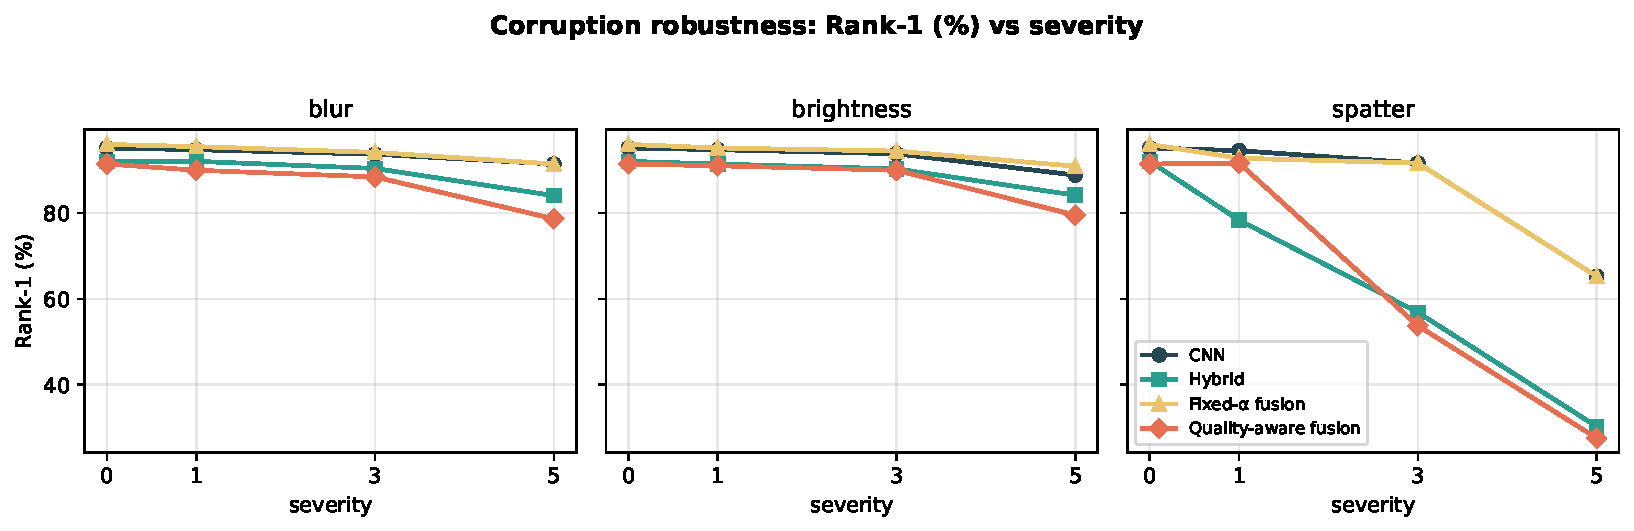
\includegraphics[width=\linewidth]{fig_corruption_rank1.pdf}
  \caption{Rank-1 vs.\ corruption severity for blur, brightness, and spatter. The
  validation-tuned fusion (yellow) tracks or exceeds the CNN across all corruptions, while
  the Hybrid and the per-sample quality-aware gate collapse under spatter (occlusion),
  because the keypoint graph is built from the clean image but the pixels are occluded.}
  \label{fig:corrupt}
\end{figure}

\Cref{tab:corrupt} and \Cref{fig:corrupt} give a clear, and partly negative, answer. The
validation-tuned scalar $\alpha$ is the best policy on \emph{all four} aggregate metrics: it
matches the CNN's clean and mean-corrupt Rank-1 while more than halving clean EER
(2.81$\to$1.17) and reducing mean-corrupt EER (4.43$\to$3.49). It achieves this by learning
$\alpha{=}0.95$ on clean and mildly corrupted data --- blending in just 5\% of the graph
branch to sharpen verification --- and $\alpha{\to}1.0$ under severe spatter, where it
gracefully abandons the fragile Hybrid and reduces exactly to the robust CNN (never worse).
The fixed $50/50$ blend, by contrast, is dragged down with the Hybrid under occlusion
(Rank-1 $33.7\%$ at spatter-5 vs.\ the CNN's $65.2\%$).

Crucially, \textbf{neither per-sample quality-adaptive policy improves on the single scalar}.
The learned gate is in fact the \emph{worst} policy for verification (clean EER $6.66\%$,
mean-corrupt $13.23\%$), and the rule-based gate is no better than the Hybrid. Per-sample
gating adds estimation variance --- each probe's $\alpha$ is noisy --- without a
correspondingly large payoff, because one branch (the CNN) dominates almost everywhere. This
is a useful negative result: for this problem, a single validation-tuned fusion weight is not
only simpler but strictly better than input-adaptive gating, mirroring our cross-domain
finding (\Cref{sec:cross}) that robust improvements come from \emph{global} score calibration
rather than fine-grained per-input adaptation.

\paragraph{Fusion ablations.} Two ablations from the plan sharpen the picture (clean test).
(i) \emph{Which complement?} Replacing the Hybrid with the pure-graph \emph{ProtoN} in the
val-tuned fusion yields the \emph{lowest} verification error of any configuration
(EER $0.67\%$, TAR@FAR=1\% $99.4\%$ at $\alpha{=}0.85$) but at a Rank-1 cost (93.6\% vs.\ the
CNN+Hybrid blend's 96.0\%), because the EER-optimal weight leans harder on the graph branch;
CNN+Hybrid remains the better \emph{ranking} fusion. (ii) \emph{Which gate features?}
Ablating the learned gate's feature groups shows the \emph{image-quality} features are what
harm it: dropping them nearly halves the gate's EER ($6.66\%\to2.95\%$), while dropping the
graph-quality or branch-disagreement features barely moves it. The gate was over-fitting
noisy per-image quality estimates on the small validation disagreement set --- yet even its
best-ablated variant (EER $2.95\%$) still loses to the trivial val-tuned scalar (EER
$1.17\%$). The negative result is thus robust to gate design.

\subsection{Explainability: A Causal Faithfulness Protocol}\label{sec:explain}
We move beyond visualisation-only explainability (Grad-CAM + attention heatmaps) to a
three-stage protocol that tests whether explanations are \emph{causally} faithful --- whether
the highlighted evidence is what the model actually uses.

\paragraph{Stage 1 --- Attribution.}
For the CNN branch we compute Grad-CAM; for the GNN branch, multi-layer GATv2 attention
rollout, graph Grad-CAM, and GNNExplainer (\texttt{src/models/explainability.py}). We
assemble a stratified case set spanning the outcome types --- correct matches, false accepts,
false rejects, and the two branch-disagreement classes (CNN-correct/GNN-wrong and
GNN-correct/CNN-wrong) --- and render side-by-side CNN-vs-GNN explanations per case
(\Cref{fig:stage1}). One case type is instructive by its rarity: only a \emph{single}
false-reject exists in the entire 964-image test set (a genuine mate scoring below the
EER threshold), a direct symptom of how well-separated the in-domain score distribution is.
Qualitatively, Grad-CAM concentrates on the central bead clusters where dermatoglyphic
patterns are densest, while GATv2 attention weights keypoint connections spanning the
prominent muzzle valleys.

\begin{figure}[t]
  \centering
  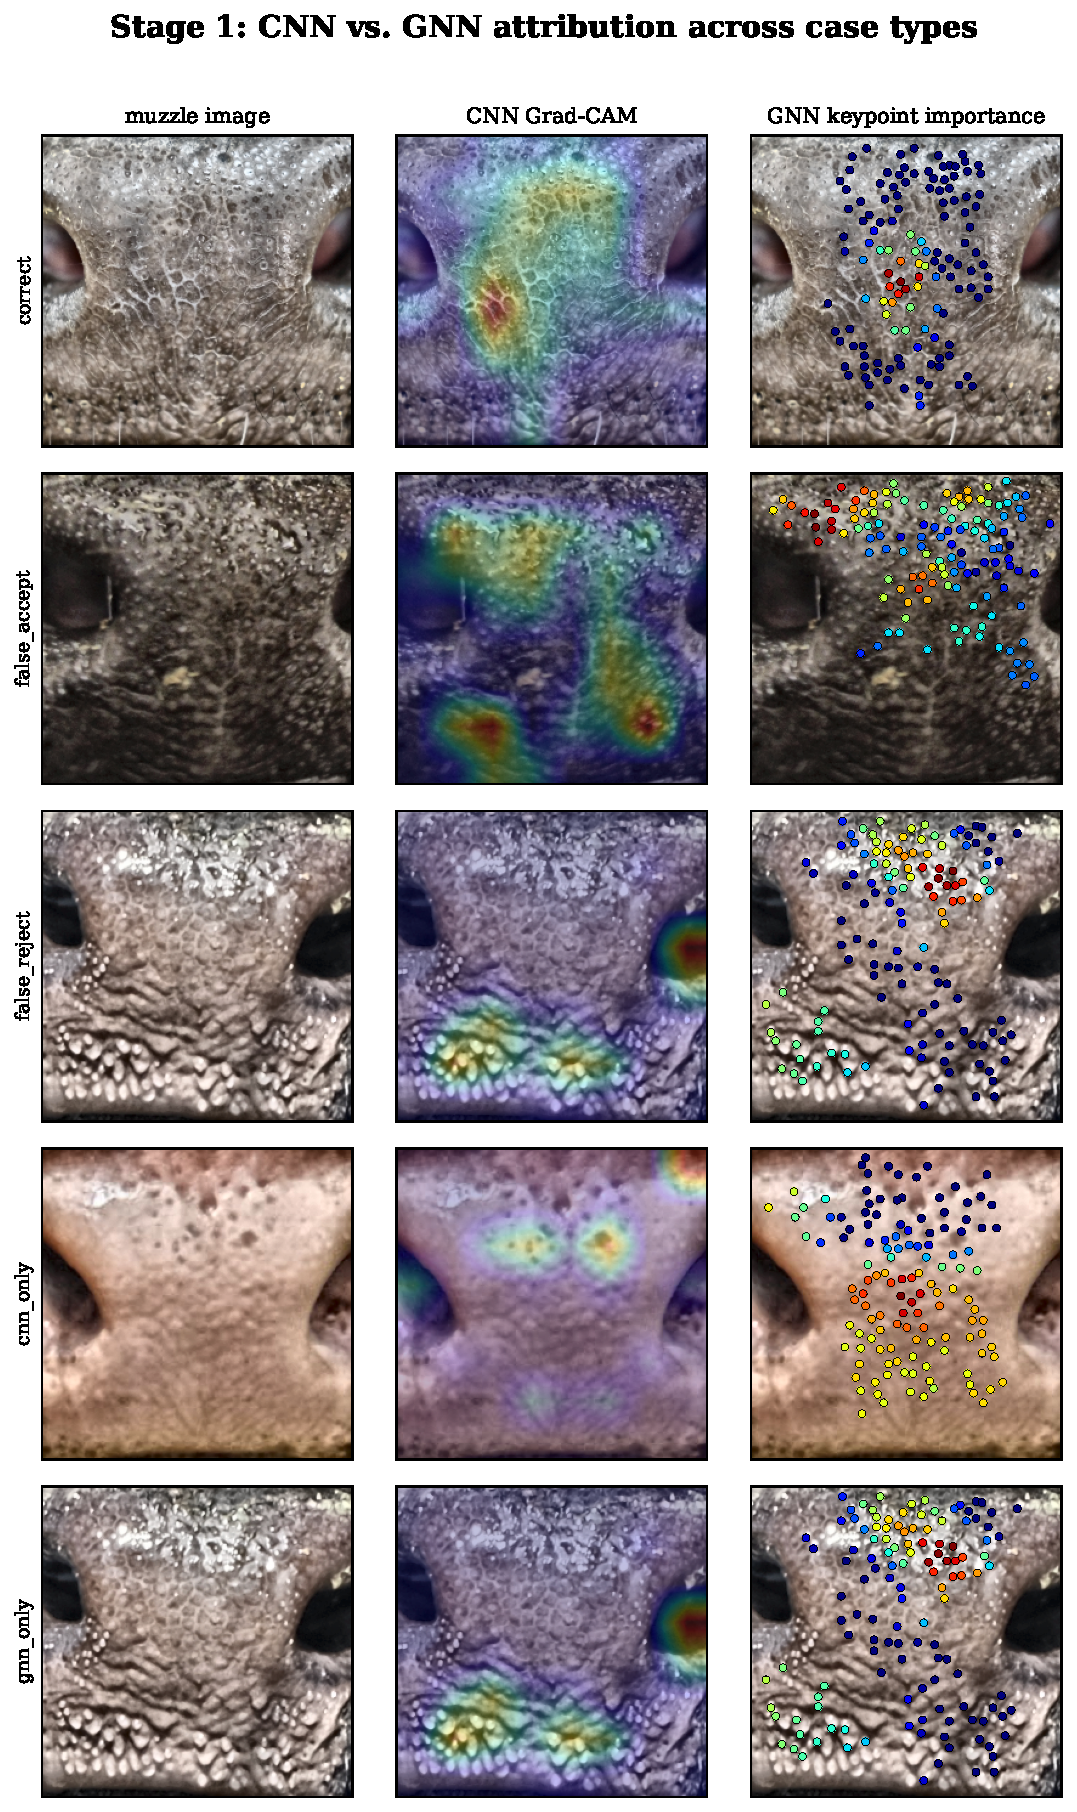
\includegraphics[width=0.86\linewidth]{fig_stage1_attribution.pdf}
  \caption{Stage 1 attribution across case types (one representative per row): the muzzle
  image, the CNN Grad-CAM heatmap, and the GNN per-keypoint importance. Both branches
  concentrate on dense dermatoglyphic bead regions; the per-keypoint GNN map is more diffuse,
  consistent with the distributed-identity finding of Stage 2.}
  \label{fig:stage1}
\end{figure}

\paragraph{Stage 2 --- Causal ablation of both branches.}
Qualitative maps are not evidence of causality. We ablate the highest-importance evidence and
measure the effect on identity, comparing against random and low-importance removal; a causally
faithful map implies \emph{top} $\gg$ \emph{random}. For the \textbf{GNN branch}
(\Cref{tab:ablation}, 120 test graphs) we rank nodes by graph Grad-CAM importance and remove
the top-/random-/bottom-$k\%$ for $k\in\{10,20,30\}$, reporting the identity-embedding shift
($\Delta\cos = 1-\cos(\text{full},\text{ablated})$, with case-resampling 95\% bootstrap CIs)
and the top-1 flip rate. The signal is clean and \emph{statistically significant}: removing
the most important nodes perturbs the embedding $2$--$2.5\times$ more than random, and the
top-vs-random $\Delta\cos$ CIs are non-overlapping at every $k$ (e.g.\ $k{=}30$:
top $[0.090,0.124]$ vs.\ random $[0.035,0.053]$). For the \textbf{CNN branch}
(\Cref{tab:ablation-cnn}, full 964-image test set) we compute Grad-CAM and mask the
top-/random-/bottom-$k\%$ of $32\times32$ image regions: masking the most important regions
causes the largest Rank-1 drop and identity flips at every $k$ (top-30\% $-5.0$ Rank-1 vs.\
random $-2.3$; flip $12.3\%$ vs.\ $5.3\%$), again with non-overlapping $\Delta\cos$ CIs.
Both branches' attributions are therefore causally faithful. One asymmetry is telling:
sparse GNN node removal barely moves closed-set Rank-1 (identity is \emph{distributed} across
many keypoints --- a global textural signature), whereas masking CNN regions produces a real,
graded Rank-1 drop.

\begin{table}[t]
  \centering
  \caption{Causal node ablation, \textbf{GNN branch} (120 test graphs; 95\% bootstrap CI on
  $\Delta\cos$). Removing Grad-CAM-\emph{important} (top) nodes shifts identity
  $\sim$2--2.5$\times$ more than random --- CIs non-overlapping at every $k$.}
  \label{tab:ablation}
  \small
  \begin{tabular}{lcc}
    \toprule
    Removed nodes & $\Delta\cos$ $\uparrow$ (95\% CI) & top-1 flip (\%) \\
    \midrule
    top 10\%    & \textbf{0.029} [0.022, 0.037] & \textbf{18.3} \\
    random 10\% & 0.013 [0.010, 0.016] & 7.5 \\
    bottom 10\% & 0.020 [0.016, 0.025] & 13.3 \\
    \midrule
    top 20\%    & \textbf{0.065} [0.053, 0.078] & \textbf{23.3} \\
    random 20\% & 0.028 [0.022, 0.036] & 14.2 \\
    bottom 20\% & 0.052 [0.043, 0.064] & 23.3 \\
    \midrule
    top 30\%    & \textbf{0.106} [0.090, 0.124] & 28.3 \\
    random 30\% & 0.043 [0.035, 0.053] & 18.3 \\
    bottom 30\% & 0.087 [0.072, 0.104] & 34.2 \\
    \bottomrule
  \end{tabular}
\end{table}

\begin{table}[t]
  \centering
  \caption{Causal region ablation, \textbf{CNN branch} (full 964-image test set). Masking
  top-importance Grad-CAM regions causes the largest Rank-1 drop and identity flips at every
  $k$ ($\Delta\cos$ CIs non-overlapping top-vs-random).}
  \label{tab:ablation-cnn}
  \small
  \begin{tabular}{lccc}
    \toprule
    Masked regions & $\Delta\cos$ $\uparrow$ & top-1 flip (\%) & Rank-1 drop \\
    \midrule
    top 10\%    & \textbf{0.0012} & \textbf{2.8} & \textbf{$-1.1$} \\
    random 10\% & 0.0007 & 1.5 & $-0.1$ \\
    bottom 10\% & 0.0009 & 2.2 & $+0.2$ \\
    \midrule
    top 20\%    & \textbf{0.0027} & \textbf{6.7} & \textbf{$-2.9$} \\
    random 20\% & 0.0018 & 3.3 & $-1.6$ \\
    bottom 20\% & 0.0024 & 3.6 & $-0.3$ \\
    \midrule
    top 30\%    & \textbf{0.0041} & \textbf{12.3} & \textbf{$-5.0$} \\
    random 30\% & 0.0028 & 5.3 & $-2.3$ \\
    bottom 30\% & 0.0038 & 5.7 & $-1.7$ \\
    \bottomrule
  \end{tabular}
\end{table}

\paragraph{Stage 3 --- Hybrid pathway intervention.}
Finally, we ask \emph{which pathway} the Hybrid relies on by perturbing its graph input at
test time and re-scoring the full test set (\Cref{tab:pathway}). The result is stark:
zeroing the per-keypoint node features collapses Rank-1 from $92.0\%$ to $0.1\%$ (EER
$1.88\%\to50.2\%$, i.e.\ chance), whereas destroying the provided graph topology (random
edges), zeroing the geometric edge attributes, or permuting the keypoint positions each moves
Rank-1 by $\le 0.5$ points. This is not an accident of the architecture but a direct
consequence of it: the Dynamic EdgeConv rebuilds its neighbourhood graph in \emph{learned
feature space} at every layer (so the static geometric edge set we supply is overridden),
the default configuration does not consume edge attributes, and the permutation-invariant
mean+max pooling makes the embedding invariant to any reindexing of the keypoints. In other
words, on clean in-domain data the Hybrid's identity signal is carried almost entirely by the
CNN texture sampled at keypoints and by feature-space message passing --- not by the input
muzzle \emph{geometry}. The same pattern holds \emph{under corruption}: repeating the
intervention on the spatter-severity-3 test set, zeroing node features still collapses Rank-1
($56.8\%\to0.1\%$) while randomising edges, zeroing edge attributes, or shuffling positions
each move it by $\le0.7$ points --- the geometry is inert whether the input is clean or
degraded. This corroborates the central finding of \Cref{sec:main} (CNN texture dominates
ranking; the graph contributes a small verification refinement) and mechanistically explains
the CNN-dominant fusion weight ($0.95$).

\paragraph{What does fusion actually rescue?} As the plan's fusion-gain measure, we tally
per-probe outcomes of the val-tuned CNN+Hybrid blend against the CNN alone on the test set.
The fusion rescues 17 probes the CNN gets wrong while harming 9 it gets right (net $+8$,
matching the $+0.9$-point Rank-1 gain), and on the 13 probes where the Hybrid is right but the
CNN is wrong it recovers 12 ($92\%$). The graph branch's contribution is thus concrete but
small and targeted --- it corrects a handful of specific CNN errors --- consistent with its
role as a verification-sharpening complement rather than a competitive ranker.

\begin{table}[t]
  \centering
  \caption{Hybrid pathway intervention (full test set). Only the per-keypoint node features
  are causally load-bearing; the supplied graph geometry is essentially inert on clean
  in-domain data.}
  \label{tab:pathway}
  \small
  \begin{tabular}{lccc}
    \toprule
    Intervention & Rank-1 (\%) & EER (\%) & $\Delta$Rank-1 \\
    \midrule
    Full Hybrid (unperturbed) & 92.0 & 1.88 & --- \\
    Zero edge attributes      & 92.0 & 1.88 & $0.0$ \\
    Shuffle keypoint positions & 92.3 & 1.84 & $-0.3$ \\
    Randomise graph edges     & 92.2 & 1.82 & $-0.2$ \\
    \textbf{Zero node features} & \textbf{0.1} & \textbf{50.2} & $\mathbf{-91.9}$ \\
    \bottomrule
  \end{tabular}
\end{table}

Together these three stages make the explainability claims falsifiable and reproducible --- the
standard we advocate for biometric-identification papers --- rather than decorative, and they
paint a consistent mechanistic picture across \Cref{sec:main}, \Cref{sec:corrupt}, and
\Cref{sec:explain}: the CNN texture pathway is the workhorse for identification, while the
graph contributes a small, calibration-like verification benefit that a single tuned weight
captures best.

% ===========================================================================
\section{Conclusion}
% ===========================================================================
We presented a comprehensive, leakage-audited evaluation of CNN, GNN, and Hybrid
architectures for cattle muzzle biometric identification. Our best single model
(EfficientNet-B4 + ArcFace) reaches 95.4\% Rank-1, and a validation-selected CNN+Hybrid
blend attains \textbf{96.1\% Rank-1} with a \textbf{0.78\% EER} --- a 3.5$\times$ reduction
in Equal Error Rate over the CNN alone. Rather than overclaiming that graphs surpass CNNs on
ranking, we localise the graph branch's value to \emph{verification robustness}, supported
by the low standalone EERs of the pure GNNs and by a controlled corruption study. We show
the representation \emph{generalises zero-shot} to two separate muzzle datasets (97.0\% and
87.0\% Rank-1, no fine-tuning; \Cref{sec:cross}) via a detector that doubles as the
deployment front-end, and that the residual cross-domain verification gap is a calibration
problem recoverable by unsupervised S-norm. We complement qualitative saliency with a
\emph{causal} explainability protocol --- statistically significant node- and region-ablation
faithfulness for both branches, and a pathway intervention showing the Hybrid's provided graph
geometry is causally inert (clean and corrupted) while identity rides on CNN texture ---
finding the GNN distributes its identity decision across many keypoints. Remaining work before camera-ready is full-budget five-fold
cross-validation of the Hybrid model and an ablation of the multi-scale node-sampling
variant; longer-term directions include cross-farm domain adaptation and low-latency on-farm
deployment.

% ===========================================================================
\section{Limitations}
% ===========================================================================
(i) The Hybrid model's cross-validation numbers (\Cref{tab:cv}) use a reduced training
budget and under-report its converged performance; full-budget CV is pending. (ii) We
evaluate open-set identification under a model trained closed-set on all identities; the
strict unseen-identity variant (retraining with unknown identities held out) is the natural
next step. (iii) Cross-dataset transfer uses a muzzle detector to crop the two external
sets; the detector missed roughly a third of images on the larger set, so those transfer
numbers are a conservative lower bound. (iv) The corruption study perturbs the image while
keypoint coordinates are taken from the clean graph, a small documented optimistic bias
under occlusion. (v) The two GNN explainers we compare show low mutual rank agreement, so
per-keypoint importance is indicative rather than definitive.

% ===========================================================================
\begin{thebibliography}{99}\small
\bibitem{arcface} J.\ Deng, J.\ Guo, N.\ Xue, S.\ Zafeiriou. ArcFace: Additive Angular Margin Loss for Deep Face Recognition. \emph{CVPR}, 2019.
\bibitem{efficientnet} M.\ Tan, Q.\ Le. EfficientNet: Rethinking Model Scaling for Convolutional Neural Networks. \emph{ICML}, 2019.
\bibitem{disk} M.\ Tyszkiewicz, P.\ Fua, E.\ Trulls. DISK: Learning Local Features with Policy Gradient. \emph{NeurIPS}, 2020.
\bibitem{gatv2} S.\ Brody, U.\ Alon, E.\ Yahav. How Attentive are Graph Attention Networks? (GATv2). \emph{ICLR}, 2022.
\bibitem{edgeconv} Y.\ Wang et al. Dynamic Graph CNN for Learning on Point Clouds (EdgeConv). \emph{ACM TOG}, 2019.
\bibitem{gnnexplainer} R.\ Ying et al. GNNExplainer: Generating Explanations for Graph Neural Networks. \emph{NeurIPS}, 2019.
\bibitem{popeexpl} P.\ Pope et al. Explainability Methods for Graph Convolutional Neural Networks. \emph{CVPR}, 2019.
\bibitem{gradcam} R.\ Selvaraju et al. Grad-CAM: Visual Explanations from Deep Networks via Gradient-based Localization. \emph{ICCV}, 2017.
\bibitem{qualityfusion} K.\ Nandakumar, Y.\ Chen, S.\ Dass, A.\ Jain. Quality-based Score Level Fusion in Multibiometric Systems. \emph{ICPR}, 2006.
\bibitem{kumar} S.\ Kumar et al. Muzzle point pattern based techniques for individual cattle identification. \emph{IET Image Processing}, 2017.
\bibitem{bello} G.\ Bello et al. Deep learning-based muzzle detection and cattle identification. 2020.
\bibitem{megadesc} V.\ \v{C}erm\'ak, L.\ Picek, L.\ Adam, K.\ Papafitsoros. WildlifeDatasets: An Open-Source Toolkit for Animal Re-Identification (MegaDescriptor). \emph{WACV}, 2024.
\bibitem{zenodo} Beef Cattle Muzzle/Noseprint Database. Zenodo, doi:10.5281/zenodo.6324361.
\bibitem{pakistan} Pakistan Cattle Muzzle/Face Dataset. Zenodo, doi:10.5281/zenodo.8377921 (CC BY 4.0).
\bibitem{yolo} G.\ Jocher et al. Ultralytics YOLOv8. 2023.
\bibitem{snorm} R.\ Auckenthaler, M.\ Carey, H.\ Lloyd-Thomas. Score Normalization for Text-Independent Speaker Verification Systems (S-norm). \emph{Digital Signal Processing}, 2000.
\bibitem{adabn} Y.\ Li, N.\ Wang, J.\ Shi, J.\ Liu, X.\ Hou. Revisiting Batch Normalization for Practical Domain Adaptation (AdaBN). \emph{ICLR Workshop}, 2017.
\end{thebibliography}

\end{document}
